\section{Context}

\begin{figure}[htb]
\centering
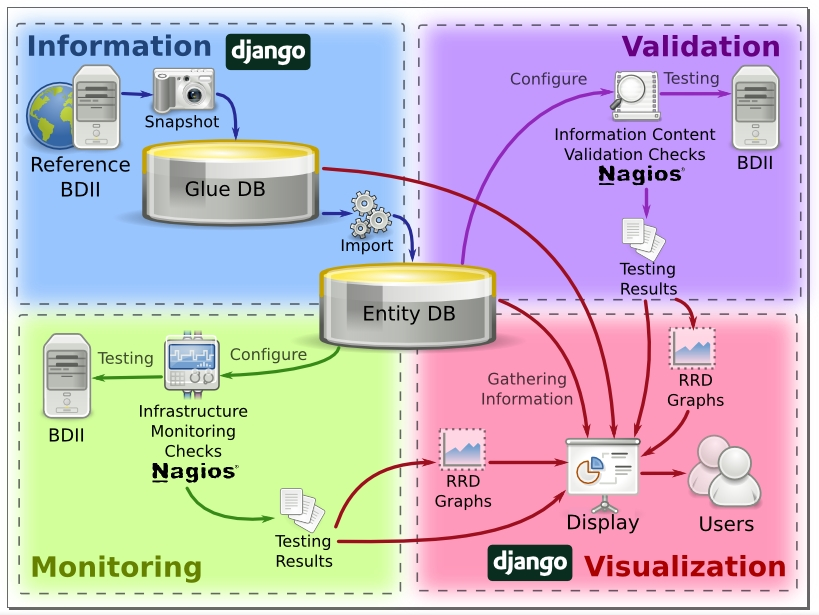
\includegraphics[width=150mm]{images/gstat-architecture.jpg}
\caption{A caption}
\label{figure:alabel}
\end{figure}

\section{Aims \& Objectives}
Different role users are going to use a portal to get information about the
performance status of the grid, to export the appropriate report for their job.
This project aims to develop these particular pieces of code to support the 
aggregation of the metrics from nagios, to allow the web based customization of
the visualization of the reports. These metrics are needed to report the
availability and reliability of NGIs and particular sites of the grid.

The procedures that are going to be used in order to achieve the above aims
should include at the beggining some opening and exploration of the environment
where the interface is going to be placed. The usage of grid computing in
the world should be well known, so a visibility of the importance and the
possible uses of the software will be recognised. The appropriate
access to the infrastructure should be gained, on different platforms and levels.
Brunel University site and GridPP/NGS VO at the beggining, as long as the UKI
ROC operations may be a good point of collaboration with researchers to reach
the bests possible requirements and data to analyse. The middleware used in
both these VOs should be examined so with the knowlege of running projects and
global usage of them may target to export better specifications. Existing
operations on the grid should also be discovered. The european initiative
milestones on the operations of the regional level should be considered as a
route, and registration to news about the upcoming research projects that
are going to use the grid should also be take place.


After that wide-opening to get the whole picture, a targeted and focused
view should follow. Existing monitoring tools must be used to check the problems
and search for requirements. The experience of SAM, Gridview, Gridmap, Gstat,
GridICE, etc should be taken in order to merge their functionality as possible
as it is. Information systems that already reside over the infrastructure, must
also be learned. Standards and specifications should be examined, on how the
message bus works and delivers the data in an hierarhical manner. A contact
with the CERN team working on MyEGEE and Indiana University's MyOSG team should
be established, to collaborate on the core of MyOSG source. Changes submission
to subversion system as long as ticket closure of the development project tool
will help to get to know the core of MyEGEE and Nagios. It is possible to create
and upstream a nagios customized web interface, to create different views of
nagios resources scheme to grid topology oriented architecture. Nagios, NRPE and
Ganglia installations should be deployed across the CE\&SE nodes of Brunel's
sites to have a working production environment to work on. Attention should be
taken on the potential performance impact of these sensors deployment. UKI
MyEGEE validation/testing portal will be used as a pre-production environment
to check changes. PNP should be fixed in GridPP Nagios to be evaluated.
Statistical access log analysis of existing tools may have results on trends of
users/admins prefered views.

Various tools are going to be used to track changes and collaborate. Monitoring
articles in GridPP wiki \& CERN twiki should be made. Snippets upstream \&
status changes must be a regular operation in SVN/JIRA/Trac in CERN interfaces.
Ongoing task through the disseration project is the reading of papers and
methodical updates of Mendeley citation management tool to have the bibliography
organized. Possible changes suggestions to MSc on DCS cource notes about grid
monitoring may by made, as long as the EGI roadmap updates. Finally with the
appropriate supervision and follow-up of meetings and presentations, a paper publishing
might take place.

\section{Organization}